\icode{N22X-EXE-FI-L3-260625-001}
\nceeID[9]{22湖南}{12}
小梦同学自制了一个两档位(“\( \times 1\)”“\( \times 10\)”)的欧姆表，其内部结构如图所示，\(R_0\)为调零电阻(最大阻值为\(R_{0 \mathrm{m}}\))，\(R_s\)、\(R_m\)、\(R_n\)为定值电阻(\(R_s + R_{0 \mathrm{m}} < R_m < R_n\))，电流计的内阻为\(R_G\)(\(R_s \ll R_G\))。用此欧姆表测量一待测电阻的阻值，回答下列问题：

\begin{figure}[htbp]
	\centering
	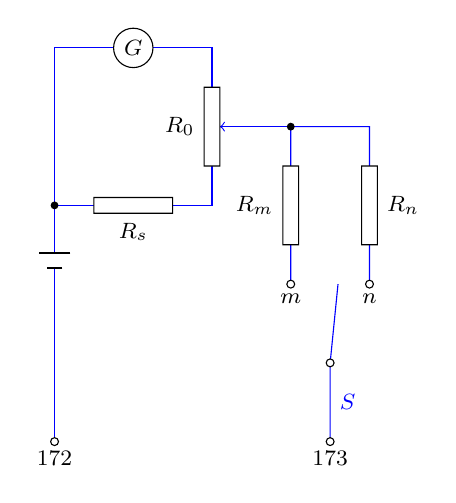
\begin{tikzpicture}[font=\footnotesize]
		\draw[blue] (0,-1)--(0,1.2) (0,1.4)--(0,4)--(2,4)--(2,2)--(0,2);
		\draw[thick] (.2,1.4)--(-.2,1.4) (.1,1.2)--(-.1,1.2);
		\draw[blue,->] (3,3)--(2.1,3);
		\draw[blue] (3,3)--(3,1) (4,1)--(4,3)--(3,3) (3.5,0)--node[right]{\(S\)}(3.5,-1) (3.5,0)--(3.6,1);
		\filldraw[fill=white] (.5,1.9) rectangle(1.5,2.1) (1.9,2.5) rectangle(2.1,3.5) (1,4)node{\(G\)} circle(.25) (2.9,1.5) rectangle(3.1,2.5) (3.9,1.5) rectangle(4.1,2.5);
		\filldraw[fill=white] (0,-1)node[below]{\ding{172}} circle(.05) (3,1)node[below]{\footnotesize \(m\)} circle(.05) (4,1)node[below]{\footnotesize \(n\)} circle(.05) (3.5,0) circle(.05) (3.5,-1)node[below]{\ding{173}} circle(.05);
		\fill (0,2) circle(.05) (3,3) circle(.05);
		\node at(1,1.9)[below]{\(R_s\)};
		\node at(1.9,3)[left]{\(R_0\)};
		\node at(2.9,2)[left]{\(R_m\)};
		\node at(4.1,2)[right]{\(R_n\)};
	\end{tikzpicture}
\end{figure}

(1)短接\ding{172}\ding{173}，将单刀双掷开关\(S\)与\(m\)接通，电流计\circled{G}示数为\(I_m\)；保持电阻\(R_0\)滑片位置不变，将单刀双掷开关\(S\)与\(n\)接通，电流计\circled{G}示数变为\(I_n\)，则\(I_m\)\lunl{4em}\(I_n\)(填“大于”或“小于”)；

(2)将单刀双掷开关\(S\)与\(n\)接触，此时欧姆表的挡位为\lunl{4em}(填“\( \times 1\)”或“\( \times 10\)”)；

(3)若从“\( \times 1\)”挡位换成“\( \times 10\)”挡位，调整欧姆零点(欧姆零点在电流计 满偏刻度处)时，调零电阻\(R_0\)的滑片应该\lunl{4em}调节(填“向上”或“向下”)；

(4)在“\( \times 10\)”挡位调整欧姆零点后，在\ding{172}\ding{173}间接入阻值为\,\qty{100}{\Omega}的定值电阻\(R_1\)，稳定后电流计\circled{G}的指针偏转到满偏刻度的\(\sfrac{2}{3}\) ；取走\(R_1\)，在\ding{172}\ding{173}间接入待测电阻\(R_x\)，稳定后电流计\circled{G}的指针偏转到满偏刻度的\(\sfrac{1}{3}\)，则\(R_x =\)\lunl{4em}\,\qty{}{\Omega}。